\chapter{مقدمه}
\label{chap:introduction}
\begin{abstract}
در این فصل  انگیزه‌ و هدفمان را، در انتخاب موضوع این رساله بیان خواهیم کرد. بدین‌منظور  نخست در
\autoref{sec:introSecTem}
به سراغ مفهوم \gls{Security} خواهیم رفت. خواهیم گفت که امروزه،
\gls{Privacy} \gls{ContextOriented}
اهمیت بی‌بدیلی در حوزه \gls{Security} یافته است. از دریای بی‌کران موضوعات مربوط به 
\gls{Privacy} \gls{ContextOriented}،
به سراغ  مبحث
 ‎\gls{TemporalAndStatisticalPrivacy} ‎ 
خواهیم رفت. برای جلب توجه خواننده به اهمیت موضوع در 
\autoref{sec:IntroApplications}،
برخی از کاربردهای مطرح در این حوزه مورد بررسی قرار خواهد گرفت. در نهایت در 
\autoref{sec:contributionIntr} و \autoref{sec:structureResale}
به ترتیب دستاوردهای حاصل گشته و ساختار رساله ارایه می‌گردد. 
\end{abstract}

\section{از \glsentrytext{Security} تا \glsentrytext{TemporalAndStatisticalPrivacy}}
\label{sec:introSecTem} \index{\glsentrytext{Security}}
\gls{Security}
از مهم‌ترین واژه‌هایی است که در فکر و ذهن بشر، از نخستین لحظات زندگانی‌اش در جریان بوده‌است. هنگامی که  ژولیوس سزار‎‎\LTRfootnote{Gaius Iulius Caesar}‎
برای نخستین بار در ۵۰ سال قبل از میلاد، رمز ساده جانشینی حرفی خود را بکار گرفت، هیچ‌گاه فکر نمی‌کرد که حوزه‌ای که در آن گام نهاده، به یکی از بزرگترین حوزه‌های تحقیقاتی دنیا مبدل خواهد شد. 
\gls{Security}
در حوالی جنگ جهانی دوم رشد شگرفی را تجربه کرد. اما آن‌چه که ما اکنون بر  آن گام می‌نهیم، مدیون دو انقلاب  بزرگ در این حوزه است، مقاله ۱۹۴۹ شانون\LTRfootnote{
Claude Elwood Shannon (April 30, 1916 – Feb 24, 2001)} \cite{Shannon1949Communication}
 و دیگری بوجود آمدن مفهوم امنیت مبتنی بر 
\gls{PublicKey} \cite{menezes1996handbook}.

تا مدت‌ها نگاه ما به 
\gls{Security}
به سه‌گانه
\gls{CIA}
خلاصه می‌گشت، اما با گذر زمان مفاهیم جدیدی نظیر
\gls{Freshness}, \gls{Nonrepudiation}, \gls{Anonymity} و \gls{Privacy}
نیز مطرح گشت و جای خود را در این حوزه پیدا کرد
\cite{menezes1996handbook}.
در این مجال، از دریای بی‌کران
\gls{Security}، به سراغ \gls{Privacy}
می‌رویم. 

\index{\glsentrytext{Privacy}}
\index{\glsentrytext{Privacy}!\glsentrytext{DataOriented}}
\index{\glsentrytext{Privacy}!\glsentrytext{ContextOriented}}
\gls{Privacy}
را می‌توان در دو دسته
\gls{DataOriented} و \gls{ContextOriented}
طبقه‌بندی نمود
\cite[بخش $12.4.1$]{guizani2015future}, \cite[صفحه 202]{mason2014sensing}.
نقطه تمرکز 
\gls{Privacy} \gls{DataOriented}،
بر روی محتوای داده است و بدین‌سان سازوکارهایی نظیر 
\gls{Encryption}, \gls{Integrity} و غیره
برای تامین چنین نیازی کارا و کافی خواهد بود. اما در این رساله به سراغ دسته دوم یعنی
\gls{Privacy} \gls{ContextOriented} 
می‌رویم.  در این دسته بالعکس دسته نخست، هدف غایی کسب اطلاعات جانبی  از داده‌ها است. فرض کنید جلسه‌ای محرمانه بین دو نفر تشکیل شده است. در این نوع از 
\gls{Privacy}،
محتوای داده (صحبت‌هایی که در جلسه مطرح شده) برای ما اهمیت ندارد، بلکه اطلاعات جانبی آن نظیر  این‌که چه‌کسانی، درکجا، کی، چگونه و چرا این جلسه را برگزار کردند، از اهمیت بیشتری برخوردار خواهد بود. 

\index{\glsentrytext{TemporalAndStatisticalPrivacy}!مفهوم}
آن‌چه که ما در این رساله به دنبال آن هستیم، نوعی از 
\gls{Privacy} \gls{ContextOriented} 
است، که ما آن را
\gls{TemporalAndStatisticalPrivacy}
می‌نامیم. در
\autoref{fig:WhatInThesis}
نسبت موضوع انتخاب گشته (یعنی 
\gls{TemporalAndStatisticalPrivacy}) 
به نسبت کل حوزه
\gls{Security}
به خوبی نشان داده شده است. خواهید دید که در
\gls{TemporalAndStatisticalPrivacy}،
 هر نوع اطلاعاتی از زمان رخداد یک حادثه چه به صورت قطعی و چه به صورت آماری (به عنوان نمونه نرخ و \gls{Variance} زمان رخداد آن حادثه) 
ممکن است 
\gls{Privacy} \gls{User}
را به مخاطره بیافکند. در ادامه برخی از کاربردهای این نوع از 
\gls{Privacy}
را ذکر خواهیم کرد.
\begin{figure}
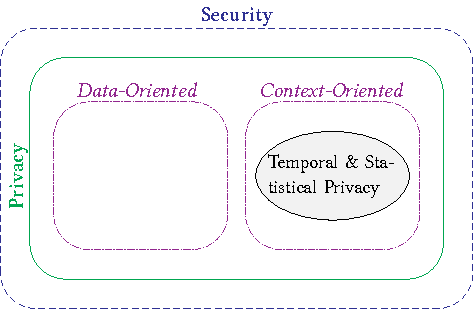
\includegraphics[width=0.6\linewidth]{Pic/WhatInThesis/mainFig}
\caption{\lofimage{Pic/WhatInThesis/mainFig}
حفظ
\gls*{Privacy}،
یکی از مهم‌ترین ابعاد حفظ
\gls*{Security} یک \gls*{System}
است. 
\gls*{Privacy} به نوبه خود به دو بخش \gls*{DataOriented} و \gls*{ContextOriented}
تقسیم‌ می‌گردد. در این رساله ما به دنبال پویش در حوزه
\gls*{TemporalAndStatisticalPrivacy} 
(از زیرمجموعه
\gls*{Privacy} \gls*{ContextOriented})
هستیم.
}
\label{fig:WhatInThesis}
\end{figure}



\section{کاربردهای \glsentrytext{TemporalAndStatisticalPrivacy}}
\index{\glsentrytext{TemporalAndStatisticalPrivacy}!کاربرد}
\label{sec:IntroApplications}
\gls*{TemporalAndStatisticalPrivacy}
از جنبه‌های بسیاری می‌تواند حائز اهمیت باشد. در ادامه ما به چند نمونه از این کاربردها اشاره خواهیم نمود. البته کاربردهای مساله یاد شده، به موضوعات مورد اشاره محدود نمی‌شود، و موارد اشاره شده تنها نمونه‌هایی از کاربردهای این حوزه هستند.

\subsection{\glsentrytext{Privacy} \glsentrytext{User} در حوزه \glsentrytext{TrafficClassification}} \index{\glsentrytext{PacketInspection}}
\index{\glsentrytext{TrafficClassification}}
تا چند سال پیش، تقریبا همه  ‎\gls{Application}هایی که بر روی رایانه‌ها اجرا می‌شدند، از پروتکل‌های شناخته شده با ‎\gls{PortNumber}‎ مشخص استفاده می‌کردند؛ به مانند
\gls{Application} \lr{FileZilla}
که از پروتکل
\gls{FTP} و \gls{PortNumber} $20$ و $21$
استفاده می‌کند. اما امروزه تعداد
‎\glspl{Application}‎ی
با پروتکل نامعلوم و اختصاصی، با ‎\gls{PortNumber}‎های غیراستاندارد و تصادفی بسیار فراگیر شده است. به عنوان نمونه‌ای از این 
\glspl{Application}‎
می‌توان از 
\lr{Skype},  \lr{BitTorrent} و \lr{VPN}
نام برد. در ضمن استفاده از سازوکارهای امنیتی در \glspl{Packet}ی تولید شده توسط کاربردهای یاد شده، موجب می‌شود که از محتوای \gls{Packet}، نتوان ‎‎‎‎پی به ‎‎\gls{Application}‎ تولید کننده آن برد. 

یک
\gls{Adversary}
بنا به جهات بسیاری تمایل دارد که دریابد که در 
\gls{SourceNode} چه \gls{Application}ی
اجرا شده است. این موضوع در حوزه‌ای از تحقیقات به نام 
\gls{TrafficClassification}‌ و یا \gls{PacketInspection}
مورد بررسی قرار می‌گیرد. روش‌های مختلفی برای کمک به \gls{Adversary} در این زمینه وجود دارد که دو نمونه از مهم‌ترین این روش‌ها به شرح زیر است
\cite{Valenti2013Reviewing} (\autoref{fig:NetworkLayers}):
\begin{figure}
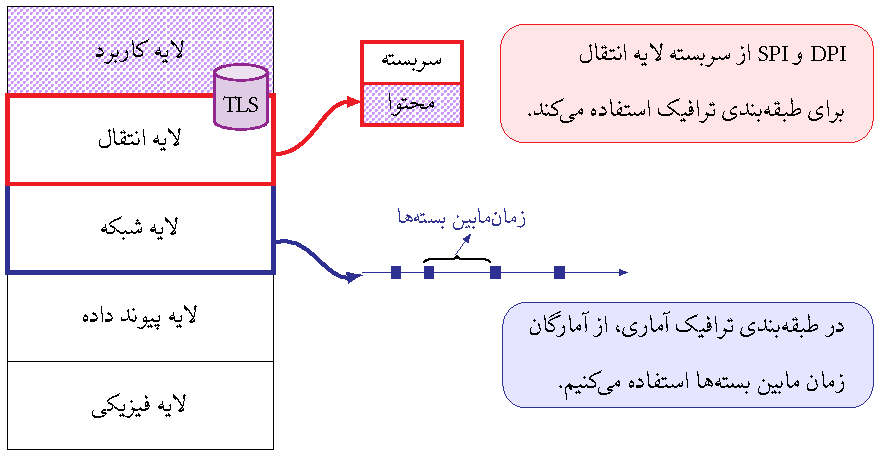
\includegraphics[width=0.75\linewidth]{Pic/NetworkLayers/mainFig}
\caption{\lofimage{Pic/NetworkLayers/mainFig}
در
\gls*{DPI} و \gls*{SPI} از محتوای \gls*{Header} \gls*{TransportLayer}
استفاده می‌شود، در حالی‌که در 
\gls*{TrafficClassification} آماری
 از آمارگان
\gls*{InterDepartureTime} \glspl*{Packet}
استفاده می‌گردد. 
}
\label{fig:NetworkLayers}
\end{figure}
\index{\glsentryname{DPI}}
\index{\glsentryname{SPI}}
\begin{itemize}
\hand \textbf{\gls{TrafficClassification}
بر مبنای ‎\gls{Payload}}‎: در این روش محتوای 
\gls{Header} \gls{TransportLayer}
 مورد بازرسی قرار می‌گیرد. در حالت کلی این روش دسته‌بندی، به دو صورت ‎\gls{DPI}‎‌ و ‎\gls{SPI}‎ انجام می‌پذیرد.
\begin{itemize}
\sci
 در ‎\gls{DPI}‎، سعی می‌شود که ‎\gls{Payload}‎ با یک امضای ثابت مقایسه گردد. دسته‌بندی بر مبنای پروتکل و ‎‎\gls{PortNumber}‎، به عنوان یکی از زیردسته‌های ‎\gls{DPI}‎ ‌محسوب می‌گردد. 
\gls{DPI}
به صورت گسترده در نرم‌افزارها و ‎\glspl{Firewall}‎ مورد استفاده قرار می‌گیرد
\cite{AbuHmed2008Survey}.
\sci

در ‎\gls{SPI}‎، ویژگی‌های آماری ‎
\gls{Header} و \gls{Payload}ی \gls{Packet} \gls{TransportLayer}،
مورد پویش قرار می‌گیرد
\cite{finamore2010kiss}.
\end{itemize}
\index{\glsentrytext{TrafficClassification}!\glsentrytext{Statistical}ی}
\hand \textbf{\gls{TrafficClassification} ‎\gls{Statistical}ی}‎:
 در این شیوه به ویژگی‌های آماری 
\gls{InterDepartureTime} و طول \glspl{Packet} در \gls{NetworkLayer}
توجه می‌شود. لازم به ذکر است که د‎ر دسته‌بندی آماری بر خلاف \gls{SPI} نیازی به بازگشایی
\gls{Packet}
وجود ندارد، بدین‌سان در این نوع از دسته‌بندی‌ حجم پردازش و محاسبات، به مراتب کمتر از 
\gls{SPI}
است. 
\end{itemize}
با زیاد شدن پروتکل‌ها،  مخفی ماندن جزئیات کارکرد آن‌ها به دلایل تجاری و استفاده از سازوکارهای امنیتی نظیر
\lr{IPSec}،
 روش‌های 
\gls{DPI} و \gls{SPI}
دیگر به خوبی نمی‌توانند جواب‌گوی ما در این مساله باشند، و بدین‌سان امروزه شاهد یک اقبال عمومی به روش‌های
\gls{TrafficClassification} ‎\gls{Statistical}ی
هستیم
\cite{Muehlstein2016Analyzing,Crotti2007Traffic}.
پرواضح است که هیچ‌کدام از ما دوست نخواهیم داشت که کسی بداند که چه
\gls{Application}ی
را در هر بازه زمانی بر روی رایانه خود اجرا می‌کنیم. این امر به نوعی جزوی از
\gls{Privacy}
ما محسوب می‌گردد. در این رساله یک چارچوب کلی برای  حفظ 
\gls{Privacy}
در مقابل این نوع از حملات ارایه می‌گردد. 


\subsection{\glsentrytext{TemporalAndStatisticalPrivacy} در \glsentryplural{WirelessSensorNetwork}}
\begin{figure}
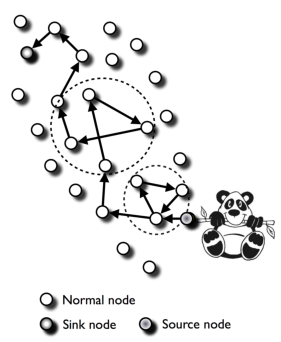
\includegraphics[width=0.45\linewidth]{./Pic/IntroductionPics/panda}
\caption[\lofimage{./Pic/IntroductionPics/panda}
حسگر‌ها به محض حس یک پاندا، گزارشی به صورت ‎\gls*{Multihop}‎ ارسال می‌کنند.]
{حسگر‌ها به محض حس یک پاندا، گزارشی به صورت ‎\gls*{Multihop}‎ ارسال می‌کنند
\cite{conti2013Providing}.}
\label{fig:panda}
\end{figure}
\lr{Ozturk}
در
\cite{Ozturk2004Source}،
مساله‌ای به نام ‎\lr{Panda-Hunter}‎ را معرفی کرده است که برطبق آن تعداد زیادی
\gls{Sensor}،
در منطقه‌ای به منظور تشخیص وجود ‎پانداها قرار داده شده است
(\autoref{fig:panda}).
هر زمان که وجود پاندایی توسط \gls{Sensor} تشخیص داده شود، سیگنالی به مرکز جمع‌آوری داده ارسال می‌گردد. 
\glspl{Sensor}
توسط پروتکل‌های
\gls{Routing} ‎\gls{Multihop}‎، 
داده خود را به دست مرکز جمع‌آوری می‌رسانند. شکارچی نیز وجود دارد که قصد دارد توسط اطلاعات ارسالی از \glspl{Sensor} به محل پاندا پی ببرد. به همین علت شکارچی  به شنود کانال منتهی به مرکز جمع‌آوری مبادرت می‌ورزد.

با رسیدن سیگنال یک \gls{Sensor} به مرکز، شکارچی در می‌یابد که اتفاقی افتاده، و بدین‌سان سعی می‌کند که مکانی که اتفاق مورد نظر رخ داده است را بیابد. از سوی دیگر، شکارچی با بدست آوردن این اطلاعات، می‌تواند نحوه رفتار حرکت پانداها را تخمین بزند، و دریابد که به احتمال زیاد در هر ساعت از شبانه‌روز، پانداها در کدام محل قرار گرفته‌اند. به نظر می‌رسد که در هر دو حالت یاد شده، مبحث ‎\gls{TemporalAndStatisticalPrivacy}‎ از اهمیت ویژه‌ای برخوردار باشد. 

\subsection{\glsentrytext{TemporalAndStatisticalPrivacy} در \glsentrytext{WBAN}}
\begin{figure}
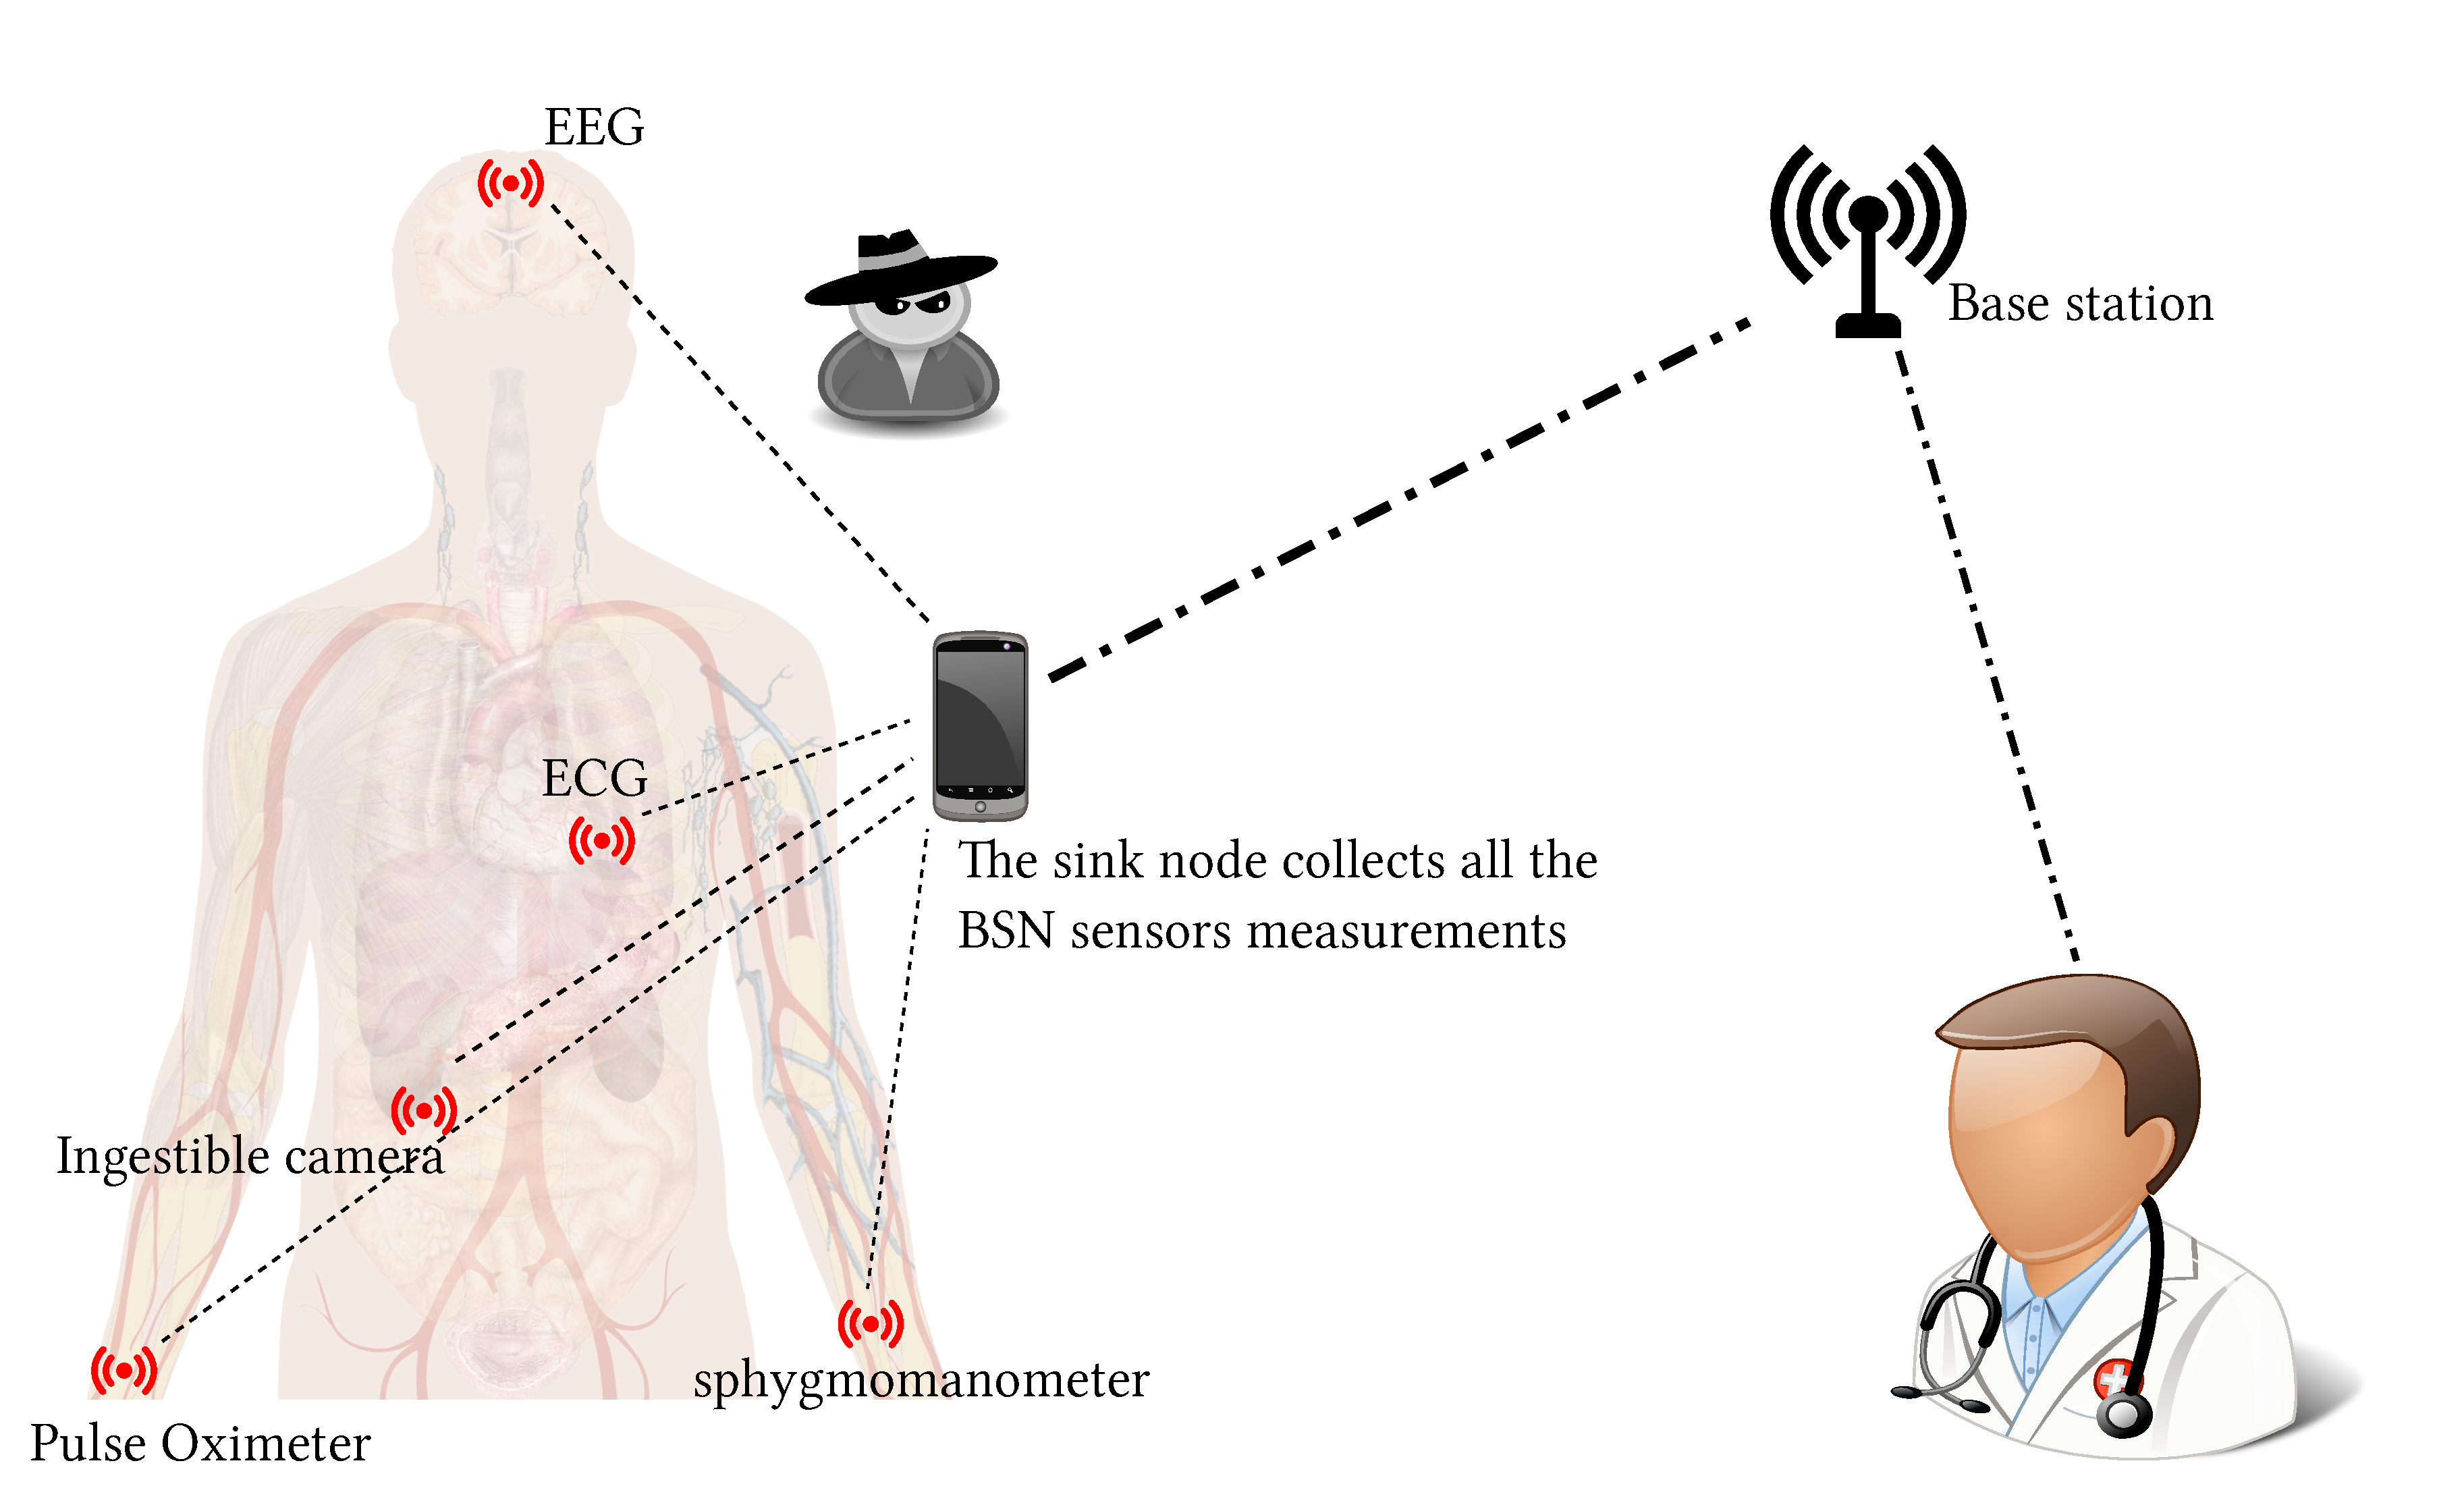
\includegraphics[width=0.7\linewidth]{Pic/IntroductionPics/WBAN}
\caption{\lofimage{Pic/IntroductionPics/WBAN}
\glspl*{Sensor}ی
نصب شده بر روی بدن بیمار در 
\gls*{WBAN}،
در زمان‌های مشخص به اندازه‌گیری علایم حیاتی او می‌پردازد. یک
\gls*{Adversary}
باهوش می‌تواند با بدست‌آوردن اطلاعات مربوط به زمان‌های اندازه‌گیری 
\glspl*{Sensor}،
پی به بیماری فرد ببرد.
}
\label{fig:WBAN}
\end{figure}
در 
\gls{WBAN} تعدادی \gls{Sensor} 
به منظور سنجش ضربان قلب، وضعیت مغز، قند، فشار، چربی و غیره، بر روی بدن بیمار  نصب می‌گردد
\cite{ullah2012comprehensive}.
بسته به نوع بیماری فرد، این 
\glspl{Sensor}
با نرخ‌های مختلفی سنجش‌های مذکور را انجام می‌دهند. به عنوان مثال فرض کنید که مریضی به علت بیماری دیابت در بیمارستان بستری شده است. پرواضح است که برای تنظیم میزان انسولین تزریقی به بیمار، نیاز است در طول روز، حداقل چهار بار میزان قند خون او سنجیده شود، در حالی‌که این تعداد اندازه‌گیری  برای سنجش چربی خون و ضربان قلب نیاز نخواهد بود. در هر بار سنجش،
\gls{Sensor}
سیگنالی را به گره مرکزی ارسال و سپس از آن‌جا این اطلاعات در صورت نیاز به پزشک معالج نیز ارایه می‌گردد.

همان‌طور که در
\autoref{fig:WBAN}
نشان داده شده، فرض کنید که یک
\gls{Adversary}
دستگاهی را در کنار تخت بیمار کار گذاشته است که هنگام ارسال سیگنال توسط هر 
\gls{Sensor}
به گره مرکزی، متوجه ارسال سیگنال می‌گردد. گرچه به علت استفاده از سازوکارهای رمزنگاری، شاید نتواند به میزان سنجه مورد اندازه‌گیری پی ببرد. اما یک
\gls{Adversary}
باهوش می‌تواند با تحلیل اطلاعات مربوط به زمان‌های ارسال سیگنال توسط هر 
\gls{Sensor}،
پی به نوع بیماری فرد ببرد. با کمی دقت می‌توان دریافت که این موضوع، به طور قطع ناقض 
\gls{Privacy}
بیمار است. 


\subsection{تشخیص \glsentrytext{Anomaly}}
فرض کنید که یک
\gls{Malware}
به رایانه شما نفوذ کرده است. نرم‌افزارهایی که برای نابودی
\glspl{Malware}
بکار گرفته می‌شوند، دو ایده کلی را دنبال می‌کنند؛ یا آن‌ها با فعالیت و نحوه تاثیر 
\gls{Malware}
آشنا هستند، و یا در صورت ناآشنا بودن با آن، به رهگیری رفتارهای غیر معمول در  \gls{OperatingSystem} می‌پردازند، و در صورت بروز چنین رفتارهایی، عامل آن رفتار را به عنوان 
\gls{Malware}
تشخیص می‌دهند
\cite{salem2008survey}.
این‌که
\gls{Malware}
به چه قسمتی از رایانه، در چه زمانی و با چه آمارگانی دسترسی پیدا می‌کند، رفتار یک
\gls{Malware}
را تشکیل می‌دهد.

بازهم ادعا می‌کنیم که چارچوب ارایه شده می‌تواند هم به 
\gls{Malware}
و هم به نگهبان رایانه شما یاری رساند. از یک سو چارچوب ارایه شده برای 
\gls{Malware}
می‌تواند مفید باشد چرا که کمک می‌کند تا اطلاعات زمانی و آماری نحوه دسترسی 
\gls{Malware}
مخفی گردد. از سوی دیگر به شما کمک می‌کند تا بتوانید ویژگی‌های زمانی و آماریی از
\gls{Malware}
استخراج نمایید که نسبت به بسیار از اتفاقاتی که در
\gls{OperatingSystem}
رخ می‌دهد، مقاوم باشد. 

\section{نوآوری‌ها}
\label{sec:contributionIntr}
در ادامه به صورت مختصر دستاوردها و نوآوری‌های بدست‌آمده در این رساله را ذکر می‌کنیم. گرچه لازم به ذکر است که هر یک از دستاوردها  متناظر با فصلی از رساله است که در جای خویش به تشریح بیان خواهد شد. 
\begin{itemize}
\sci
در
\autoref{chap:ratePrivacy}،
روشی پیشنهاد خواهیم داد که در آن با استفاده از اضافه کردن تعدادی بسته که ما از آن‌ها با عنوان
 \glspl{DummyPacket}
یاد می‌کنیم، سعی داریم که 
\gls{Privacy} \gls{Rate}
را حفظ کنیم. لازم به ذکر است که در روش پیشنهادی به منظور حفظ
\gls{QoS}،
تنها تعدادی بسته اضافه خواهد گشت و بسته‌ای حذف نخواهد شد. در همان فصل خواهید دید که با استفاده از 
\gls{FanoSInequality} \cite[قضیه $2.10.1$]{cover2006elements}،
معیاری برای توصیف ریاضیاتی
\gls{Privacy}
پیشنهاد خواهیم داد. سپس با یاری‌جستن از یک 
\gls{OptimizationProblem}، \gls{TradeOff} بین \gls{Privacy} و \gls{CommunicationCost}‌ناشی از ارسال
 \glspl{DummyPacket}،
مدیریت خواهد شد. در 
\autoref{sec:contribution}،
به صورت جزئی‌تر به تشریح دستاوردهای حاصل گشته در این قسمت، مبادرت خواهیم ورزید. در ضمن مطالب بیان شده، در مقاله زیر نیز ارایه گشته است. 
\begin{latin}
\baselineskip=.8cm
A. Diyanat, A. Khonsari, and S. P. Shariatpanahi, “A Dummy-Based Approach for Preserving Source Rate Privacy,” \textit{IEEE Transactions on Information Forensics and Security}, vol. 11, no. 6, pp. 1321–1332, Jun. 2016.
\end{latin}
\sci
در
\autoref{chap:FeaturePrivacy}،
توسعه‌ای همه‌جانبه بر مطالب
\autoref{chap:ratePrivacy}
خواهیم داشت. اولا خود را محدود به \gls{Rate} نخواهیم کرد، و به صورت کلی در مورد حفظ 
\gls{Privacy} یک \gls{Feature}
صحبت خواهیم نمود.  ثانیا 
\gls{Mapping}
بین 
\glspl{Feature}
به صورت کلی در نظر گرفته می‌شود؛ به عبارت‌بهتر اگر
\gls{Feature} را همان \gls{Rate}
در نظر بگیریم، هم می‌توان با اضافه کردن
\glspl{DummyPacket}، به \gls{Rate}
اضافه کرد و هم با حذف برخی از 
\glspl{Packet}، از \gls{Rate}
کاست.  در ضمن فرضی نیز بر روی توزیع اجرای 
\glspl{Application}
نخواهیم داشت. از سوی دیگر سه 
\gls{LowerBound} به منظور توصیف \gls{AdversarysBestEstimationErrorProbability}
با بهره‌گیری از علم
\gls{InformationTheory}
بکار گرفته می‌شود. ضمن تشریح نوآوری بدست آمده در این فصل در 
\autoref{sec:contributionExt}،
این مطالب در مقاله زیر نیز ارایه گشته است. 
\begin{latin}
\baselineskip=.8cm
A. H. RezaeiTabar, A. Diyanat, and A. Khonsari, “On the Perfect Privacy: a Statistical Analysis of Network Traffic Approach,” \textit{IEEE Communications Letters}, pp. 1–4, 2016.
\end{latin}
\sci
در 
\autoref{chap:privacyInCaching}،
به سراغ 
\glspl{CachingSystem}
خواهیم رفت. در آن‌جا ذکر خواهد شد که اگر یک
\gls{Adversary}
باهوش، به شنود 
\gls{Link}
ارتباطی بین
\gls{AP} تا \gls{Server}
بپردازد، می‌تواند در مرحله
\gls{Delivery} داده،
پی ببرد که \gls{User} کدام فایل را درخواست کرده، و بدین‌سان
\gls{Privacy} \gls{User}
نقض خواهد شد. در فصل مذکور با طرح یک 
\gls{OptimizationProblem}
خواهیم گفت که چگونه می‌توان 
\gls{Policy} \gls{Optimal}ای برای نحوه پر کردن \glspl{Cache}
یافت به‌گونه‌ای که هم 
\gls{Privacy}
حفظ شود و هم میزان ترافیک مبادله شده در مرحله
\gls{Delivery}
کاهش یابد. از سوی دیگر کمی نمودن 
\gls{Privacy}‌در \glspl{CachingSystem}
نیز از جمله نوآوری‌های مهم در این فصل خواهد بود. نوآوری‌های ارایه شده در این قسمت به صورت دقیق‌تر در 
\autoref{sec:contributionCache} و مقاله زیر
تشریح شده است. 
\begin{latin}
\baselineskip=.8cm
A. Diyanat, A. Khonsari, and S. P. Shariatpanahi, “An Information Theoretic Approach to Evaluate and Preserve Privacy in a Network Caching System,” \textit{Submitted in ACM MobiHoc 2017}, 2016.
\end{latin}
\sci
در 
\autoref{chapter:WBSNPrivacy}،
به سراغ یک شبکه 
\gls{WBSN}
خواهیم رفت. بیان خواهد شد که 
\gls{Adversary}
با دست‌یابی به اطلاعات جانبی داده‌ها بین گره کنترل‌کننده و 
\glspl{Sensor} در یک شبکه \gls{WBSN}،
می‌تواند 
\gls{Privacy}
بیمار را به خطر بیافکند. در ضمن همان‌طور که خواهد گذشت، ما برای حل این چالش، ایده‌ای مبتنی بر 
\glspl{TimeDependentPriorityQueue}
ارایه خواهیم داد. در ضمن شایان ذکر است که مفهوم
\glspl{TimeDependentPriorityQueue}
نیز برای 
\glspl{PriorityFunction}
عمومی گسترش خواهد یافت. مطالب بیان شده در این فصل در مقاله زیر ارایه شده است. 
\begin{latin}
\baselineskip=.8cm
A. Diyanat, A. Khonsari, and S. H. Shafiei, “Preservation of Temporal Privacy in Body Sensor
Networks,” \textit{Journal of Network and Computer Applications - Elsevier}, 2017.
\end{latin}
\end{itemize}

\section{ساختار رساله}
\label{sec:structureResale}
حاصل کار پژوهشی این رساله در شش فصل و یک پیوست جمع‌آوری شده است. بعد از مطالب مقدماتی که در این فصل ذکر شد، در
\autoref{chap:realtedWork}،
گذری بر کارهای تحقیقاتی خواهیم داشت که از جنبه‌های مختلف با موضوع رساله در ارتباط هستند.  
در
\autoref{chap:ratePrivacy}،
چارچوبی ارایه می‌گردد که توسط آن می‌توان 
\gls{Privacy} \gls{Rate}
را حفظ نمود. 
\autoref{chap:FeaturePrivacy}
به نوعی گسترش و توسعه همه‌جانبه مطالب
\autoref{chap:ratePrivacy}
خواهد بود. در 
\autoref{chap:privacyInCaching}
نیز به سراغ 
\gls{Privacy} \glspl{CachingSystem}
خواهیم رفت. در 
\autoref{chapter:WBSNPrivacy} نیز \gls{Privacy} در \gls{WBSN}
بررسی می‌گردد. در نهایت نیز در 
\autoref{chap:futureWork}،
نتیجه رساله به همراه پیشنهاداتی برای کارهای آتی ذکر خواهد شد. 



